\begin{figure}[tbp]
\centering
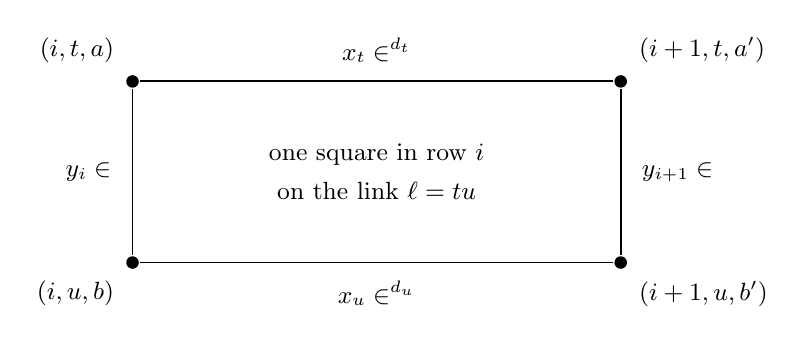
\begin{tikzpicture}[x=1cm,y=1cm,line width=.7pt,font=\small]
 \node[circle,fill,inner sep=1.6pt] (tl) at (0,0) {};
 \node[circle,fill,inner sep=1.6pt] (tr) at (6.2,0) {};
 \node[circle,fill,inner sep=1.6pt] (bl) at (0,-2.3) {};
 \node[circle,fill,inner sep=1.6pt] (br) at (6.2,-2.3) {};
 \draw (tl) -- node[above=3pt] {\(x_t\in\F^{d_t}\)} (tr);
 \draw (bl) -- node[below=3pt] {\(x_u\in\F^{d_u}\)} (br);
 \draw (tl) -- node[left=4pt] {\(y_i\in\F\)} (bl);
 \draw (tr) -- node[right=4pt] {\(y_{i+1}\in\F\)} (br);
 \node[above left=3pt] at (tl) {\((i,t,a)\)};
 \node[above right=3pt] at (tr) {\((i+1,t,a')\)};
 \node[below left=3pt] at (bl) {\((i,u,b)\)};
 \node[below right=3pt] at (br) {\((i+1,u,b')\)};
 \node[align=center] at (3.1,-1.15)
   {one square in row \(i\)\\[3pt]on the link \(\ell=tu\)};
\end{tikzpicture}
\caption{The corner diagram of a single square. The side labels satisfy
\((a,b)\in\cM_{\ell,i}\) and
\((a',b')\in\cM_{\ell,i+1}\). The horizontal readouts are vector-valued;
the vertical readouts are scalar.
These corners belong to the affine data; the output-graph vertices are
introduced in the next section.}
\label{offset:fig-square}
\end{figure}
